\begin{minipage}{0.55\textwidth}
    \begin{figure}[h]
    \centering
    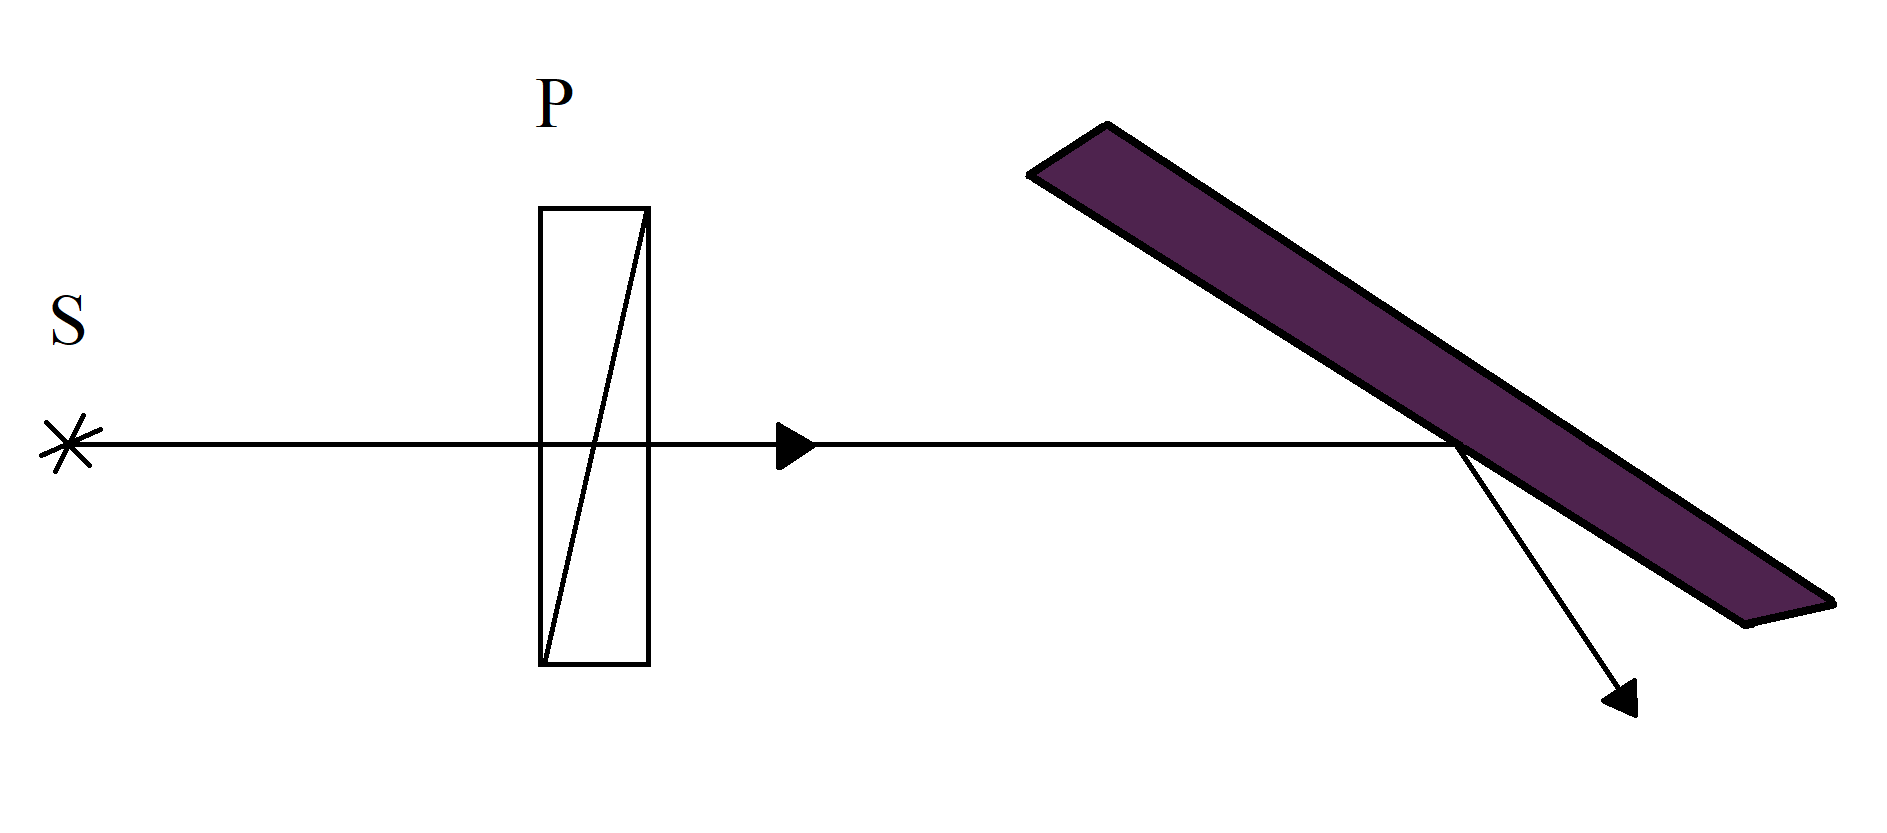
\includegraphics[width=1\textwidth]{images/mirror.png}
    \caption{We put a polaroid P and a mirror (violet one) on the way of light.}
    %\label{fig:}
\end{figure}
\end{minipage}
\hfill
\begin{minipage}{0.35\textwidth}
	Now we can make a rough estimation of polarization direction. And by adding the second polaroid we can also etimate it's polarization direction.
	\begin{align*}
		&P_1 \colon -4^\circ&\\
		&P_2 \colon 291^\circ&
	\end{align*}
\end{minipage}

